\begin{figure}
    \centering
    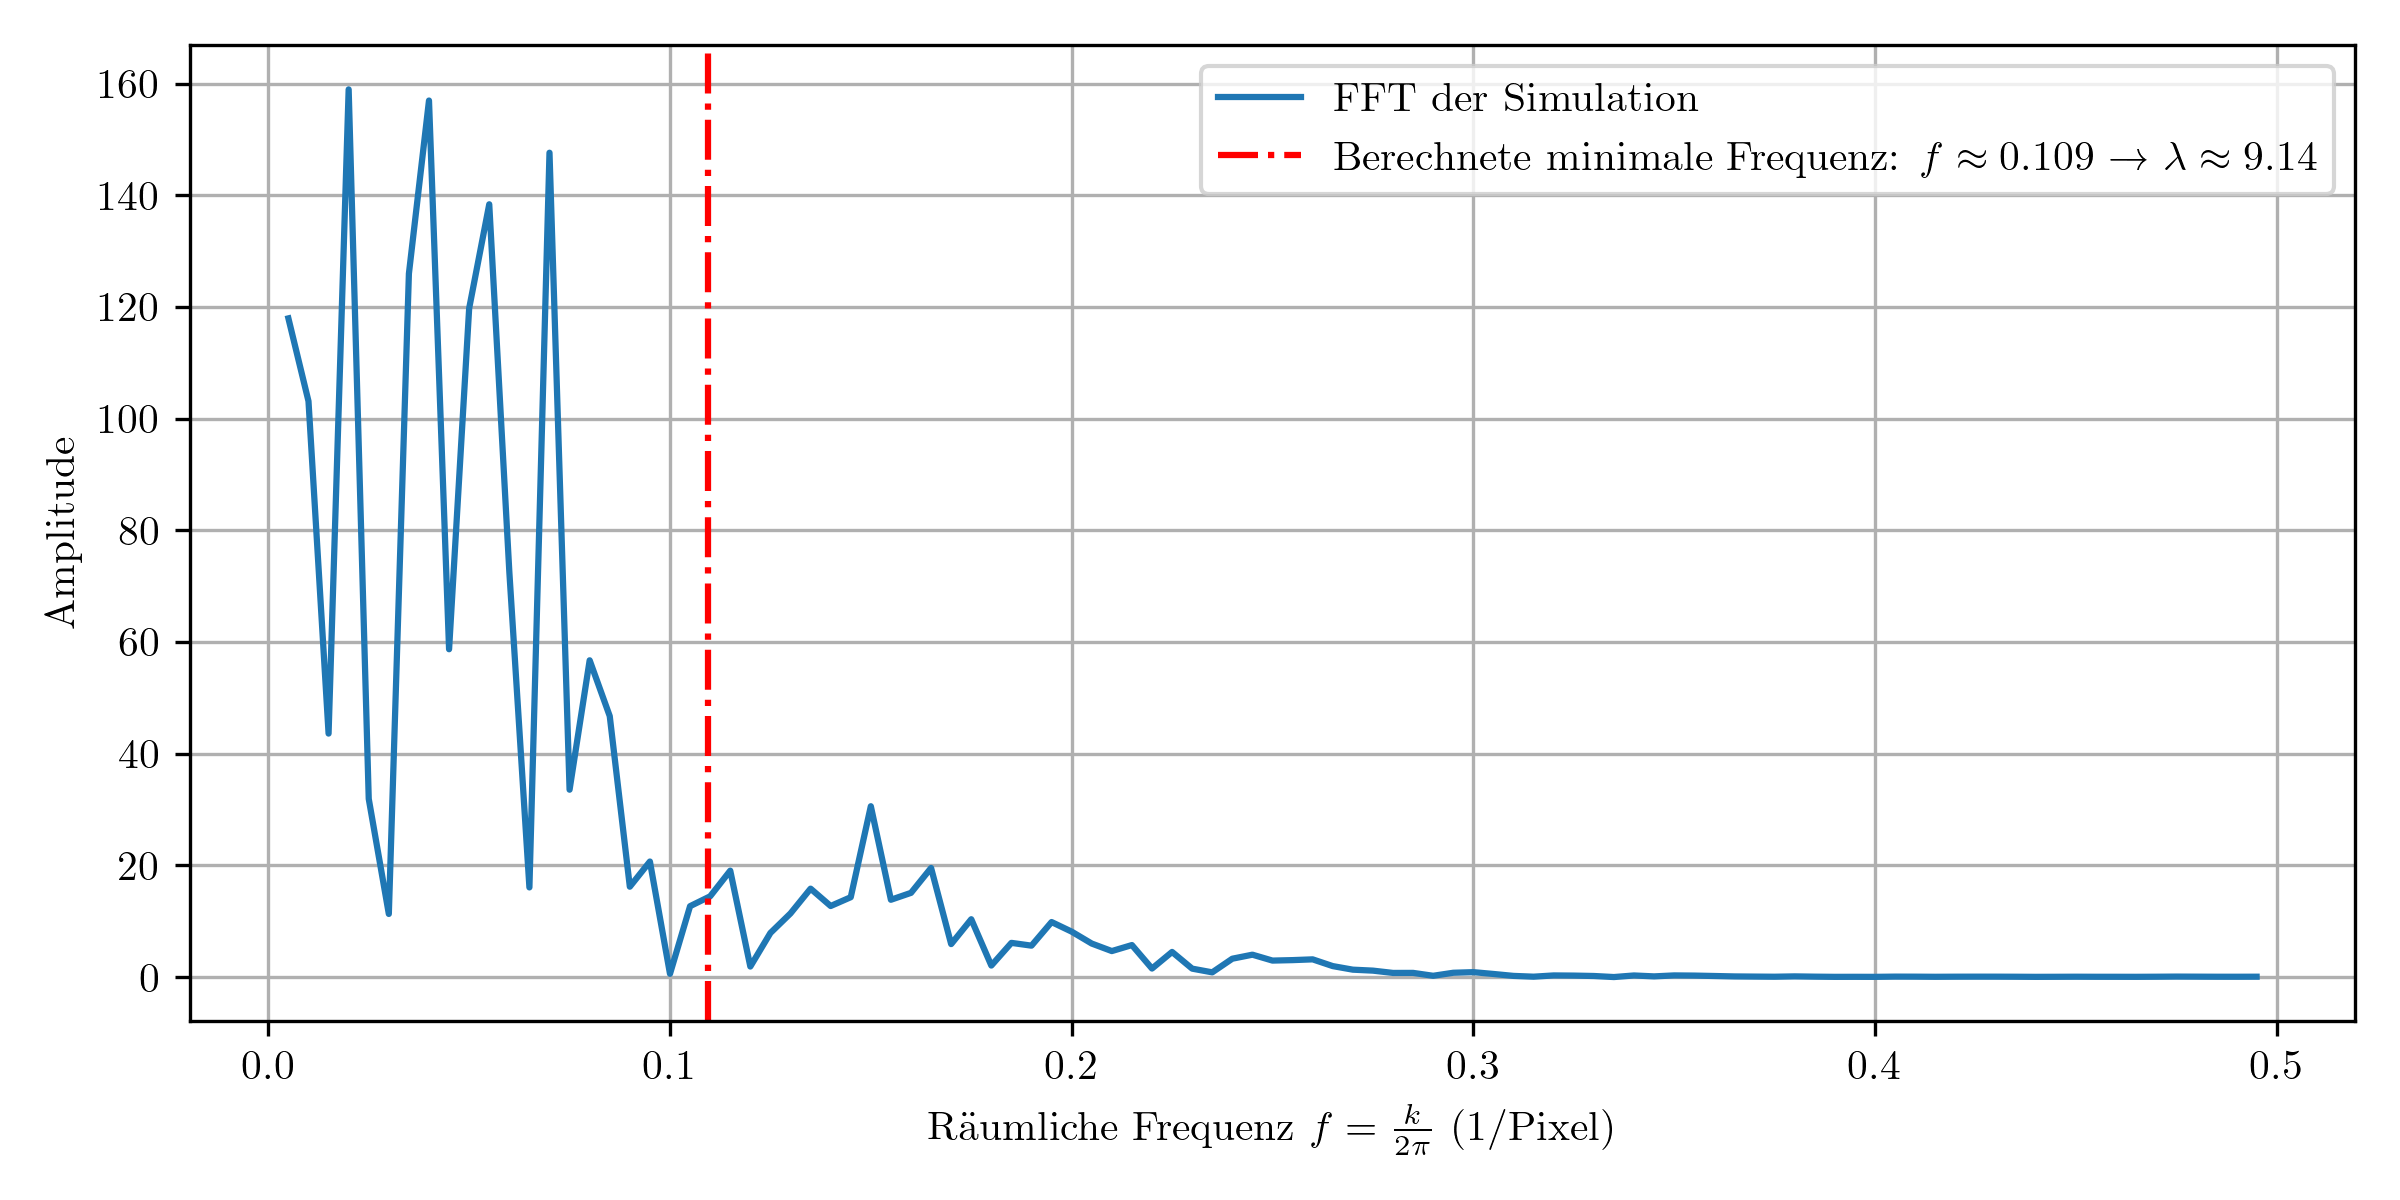
\includegraphics[width=\linewidth]{papers/reaktdiff/images/simpleExample/fft_turing_1d.png}
    \caption{FFT der Simulation eines Reaktionsdiffusionsmodell mit linearen Reaktionstermen \eqref{reaktdiff:equ:ownreakterm}. Die rote Linie zeigt die theortische minimale Frequnez von \(f = k_{\min} / 2 \pi \approx 0.109\). Man sieht, dass die dominanten Frequenzen links des berechneten Minimums ist.}
    \label{reaktdiff:fig:easyfft}
\end{figure}
